% Created by tikzDevice version 0.12.4 on 2023-11-06 21:01:34
% !TEX encoding = UTF-8 Unicode
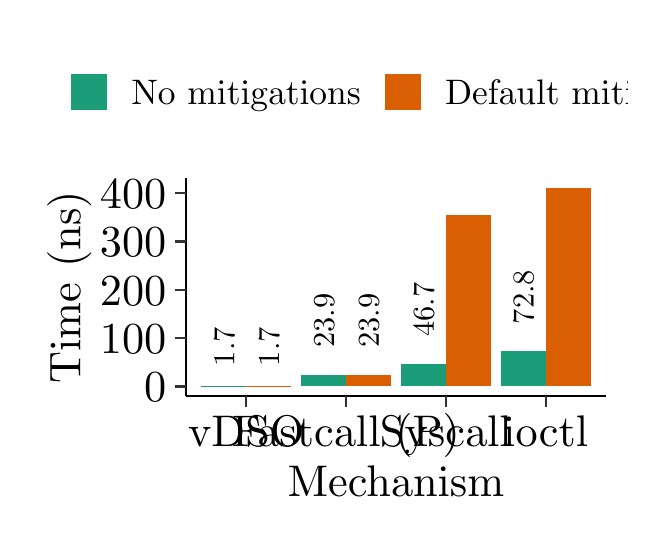
\begin{tikzpicture}[x=1pt,y=1pt]
\definecolor{fillColor}{RGB}{255,255,255}
\path[use as bounding box,fill=fillColor,fill opacity=0.00] (0,0) rectangle (216.81,180.67);
\begin{scope}
\path[clip] (  0.00,  0.00) rectangle (216.81,180.67);
\definecolor{drawColor}{RGB}{255,255,255}
\definecolor{fillColor}{RGB}{255,255,255}

\path[draw=drawColor,line width= 0.8pt,line join=round,line cap=round,fill=fillColor] ( -0.00,  0.00) rectangle (216.81,180.67);
\end{scope}
\begin{scope}
\path[clip] ( 57.32, 47.46) rectangle (208.81,126.22);
\definecolor{fillColor}{RGB}{255,255,255}

\path[fill=fillColor] ( 57.32, 47.46) rectangle (208.81,126.22);
\definecolor{fillColor}{RGB}{217,95,2}

\path[fill=fillColor] (187.17, 51.04) rectangle (203.40,122.64);

\path[fill=fillColor] (151.10, 51.04) rectangle (167.33,113.08);

\path[fill=fillColor] (115.03, 51.04) rectangle (131.26, 55.21);

\path[fill=fillColor] ( 78.96, 51.04) rectangle ( 95.20, 51.33);
\definecolor{fillColor}{RGB}{27,158,119}

\path[fill=fillColor] (170.94, 51.04) rectangle (187.17, 63.73);

\path[fill=fillColor] (134.87, 51.04) rectangle (151.10, 59.19);

\path[fill=fillColor] ( 98.80, 51.04) rectangle (115.03, 55.21);

\path[fill=fillColor] ( 62.73, 51.04) rectangle ( 78.96, 51.33);
\definecolor{drawColor}{RGB}{0,0,0}

\node[text=drawColor,rotate= 90.00,anchor=base west,inner sep=0pt, outer sep=0pt, scale=  1.10] at (199.09,135.21) {410.5};

\node[text=drawColor,rotate= 90.00,anchor=base west,inner sep=0pt, outer sep=0pt, scale=  1.10] at (163.02,125.65) {355.7};

\node[text=drawColor,rotate= 90.00,anchor=base west,inner sep=0pt, outer sep=0pt, scale=  1.10] at (126.95, 65.03) {23.9};

\node[text=drawColor,rotate= 90.00,anchor=base west,inner sep=0pt, outer sep=0pt, scale=  1.10] at ( 90.88, 58.38) {1.7};

\node[text=drawColor,rotate= 90.00,anchor=base west,inner sep=0pt, outer sep=0pt, scale=  1.10] at (182.86, 73.54) {72.8};

\node[text=drawColor,rotate= 90.00,anchor=base west,inner sep=0pt, outer sep=0pt, scale=  1.10] at (146.79, 69.00) {46.7};

\node[text=drawColor,rotate= 90.00,anchor=base west,inner sep=0pt, outer sep=0pt, scale=  1.10] at (110.72, 65.02) {23.9};

\node[text=drawColor,rotate= 90.00,anchor=base west,inner sep=0pt, outer sep=0pt, scale=  1.10] at ( 74.65, 58.38) {1.7};
\end{scope}
\begin{scope}
\path[clip] (  0.00,  0.00) rectangle (216.81,180.67);
\definecolor{drawColor}{RGB}{0,0,0}

\path[draw=drawColor,line width= 0.6pt,line join=round] ( 57.32, 47.46) --
	( 57.32,126.22);
\end{scope}
\begin{scope}
\path[clip] (  0.00,  0.00) rectangle (216.81,180.67);
\definecolor{drawColor}{RGB}{0,0,0}

\node[text=drawColor,anchor=base east,inner sep=0pt, outer sep=0pt, scale=  1.60] at ( 50.12, 45.53) {0};

\node[text=drawColor,anchor=base east,inner sep=0pt, outer sep=0pt, scale=  1.60] at ( 50.12, 62.97) {100};

\node[text=drawColor,anchor=base east,inner sep=0pt, outer sep=0pt, scale=  1.60] at ( 50.12, 80.41) {200};

\node[text=drawColor,anchor=base east,inner sep=0pt, outer sep=0pt, scale=  1.60] at ( 50.12, 97.86) {300};

\node[text=drawColor,anchor=base east,inner sep=0pt, outer sep=0pt, scale=  1.60] at ( 50.12,115.30) {400};
\end{scope}
\begin{scope}
\path[clip] (  0.00,  0.00) rectangle (216.81,180.67);
\definecolor{drawColor}{gray}{0.20}

\path[draw=drawColor,line width= 0.8pt,line join=round] ( 53.32, 51.04) --
	( 57.32, 51.04);

\path[draw=drawColor,line width= 0.8pt,line join=round] ( 53.32, 68.48) --
	( 57.32, 68.48);

\path[draw=drawColor,line width= 0.8pt,line join=round] ( 53.32, 85.92) --
	( 57.32, 85.92);

\path[draw=drawColor,line width= 0.8pt,line join=round] ( 53.32,103.37) --
	( 57.32,103.37);

\path[draw=drawColor,line width= 0.8pt,line join=round] ( 53.32,120.81) --
	( 57.32,120.81);
\end{scope}
\begin{scope}
\path[clip] (  0.00,  0.00) rectangle (216.81,180.67);
\definecolor{drawColor}{RGB}{0,0,0}

\path[draw=drawColor,line width= 0.6pt,line join=round] ( 57.32, 47.46) --
	(208.81, 47.46);
\end{scope}
\begin{scope}
\path[clip] (  0.00,  0.00) rectangle (216.81,180.67);
\definecolor{drawColor}{gray}{0.20}

\path[draw=drawColor,line width= 0.8pt,line join=round] ( 78.96, 43.46) --
	( 78.96, 47.46);

\path[draw=drawColor,line width= 0.8pt,line join=round] (115.03, 43.46) --
	(115.03, 47.46);

\path[draw=drawColor,line width= 0.8pt,line join=round] (151.10, 43.46) --
	(151.10, 47.46);

\path[draw=drawColor,line width= 0.8pt,line join=round] (187.17, 43.46) --
	(187.17, 47.46);
\end{scope}
\begin{scope}
\path[clip] (  0.00,  0.00) rectangle (216.81,180.67);
\definecolor{drawColor}{RGB}{0,0,0}

\node[text=drawColor,anchor=base,inner sep=0pt, outer sep=0pt, scale=  1.60] at ( 78.96, 29.24) {vDSO};

\node[text=drawColor,anchor=base,inner sep=0pt, outer sep=0pt, scale=  1.60] at (115.03, 29.24) {Fastcall (P)};

\node[text=drawColor,anchor=base,inner sep=0pt, outer sep=0pt, scale=  1.60] at (151.10, 29.24) {Syscall};

\node[text=drawColor,anchor=base,inner sep=0pt, outer sep=0pt, scale=  1.60] at (187.17, 29.24) {ioctl};
\end{scope}
\begin{scope}
\path[clip] (  0.00,  0.00) rectangle (216.81,180.67);
\definecolor{drawColor}{RGB}{0,0,0}

\node[text=drawColor,anchor=base,inner sep=0pt, outer sep=0pt, scale=  1.60] at (133.07, 11.11) {Mechanism};
\end{scope}
\begin{scope}
\path[clip] (  0.00,  0.00) rectangle (216.81,180.67);
\definecolor{drawColor}{RGB}{0,0,0}

\node[text=drawColor,rotate= 90.00,anchor=base,inner sep=0pt, outer sep=0pt, scale=  1.60] at ( 19.02, 86.84) {Time (ns)};
\end{scope}
\begin{scope}
\path[clip] (  0.00,  0.00) rectangle (216.81,180.67);
\definecolor{fillColor}{RGB}{255,255,255}

\path[fill=fillColor] ( -0.99,142.22) rectangle (267.12,172.67);
\end{scope}
\begin{scope}
\path[clip] (  0.00,  0.00) rectangle (216.81,180.67);
\definecolor{fillColor}{RGB}{27,158,119}

\path[fill=fillColor] ( 15.72,150.93) rectangle ( 28.75,163.96);
\end{scope}
\begin{scope}
\path[clip] (  0.00,  0.00) rectangle (216.81,180.67);
\definecolor{fillColor}{RGB}{217,95,2}

\path[fill=fillColor] (129.07,150.93) rectangle (142.10,163.96);
\end{scope}
\begin{scope}
\path[clip] (  0.00,  0.00) rectangle (216.81,180.67);
\definecolor{drawColor}{RGB}{0,0,0}

\node[text=drawColor,anchor=base west,inner sep=0pt, outer sep=0pt, scale=  1.28] at ( 37.46,153.04) {No mitigations};
\end{scope}
\begin{scope}
\path[clip] (  0.00,  0.00) rectangle (216.81,180.67);
\definecolor{drawColor}{RGB}{0,0,0}

\node[text=drawColor,anchor=base west,inner sep=0pt, outer sep=0pt, scale=  1.28] at (150.81,153.04) {Default mitigations};
\end{scope}
\end{tikzpicture}
